\section{Atmos}

The race car that Revolve NTNU is trying to make autonomous is called Atmos. It was built last year as that years electrical car. Now it is being refitted with all the sensors needed for acting without human input. Below some of the necessary language needed for the further discussion is explained. Then the sensors on the car are explained; what sensors there are, how they work and what information they give. A brief introduction to the cone detection algorithms is then given. Finally last years solutions to the problems that this thesis tries to solve are explained.

Atmos is seen in figure \ref{Fig:Atmos}.

\begin{figure}
    \centering
    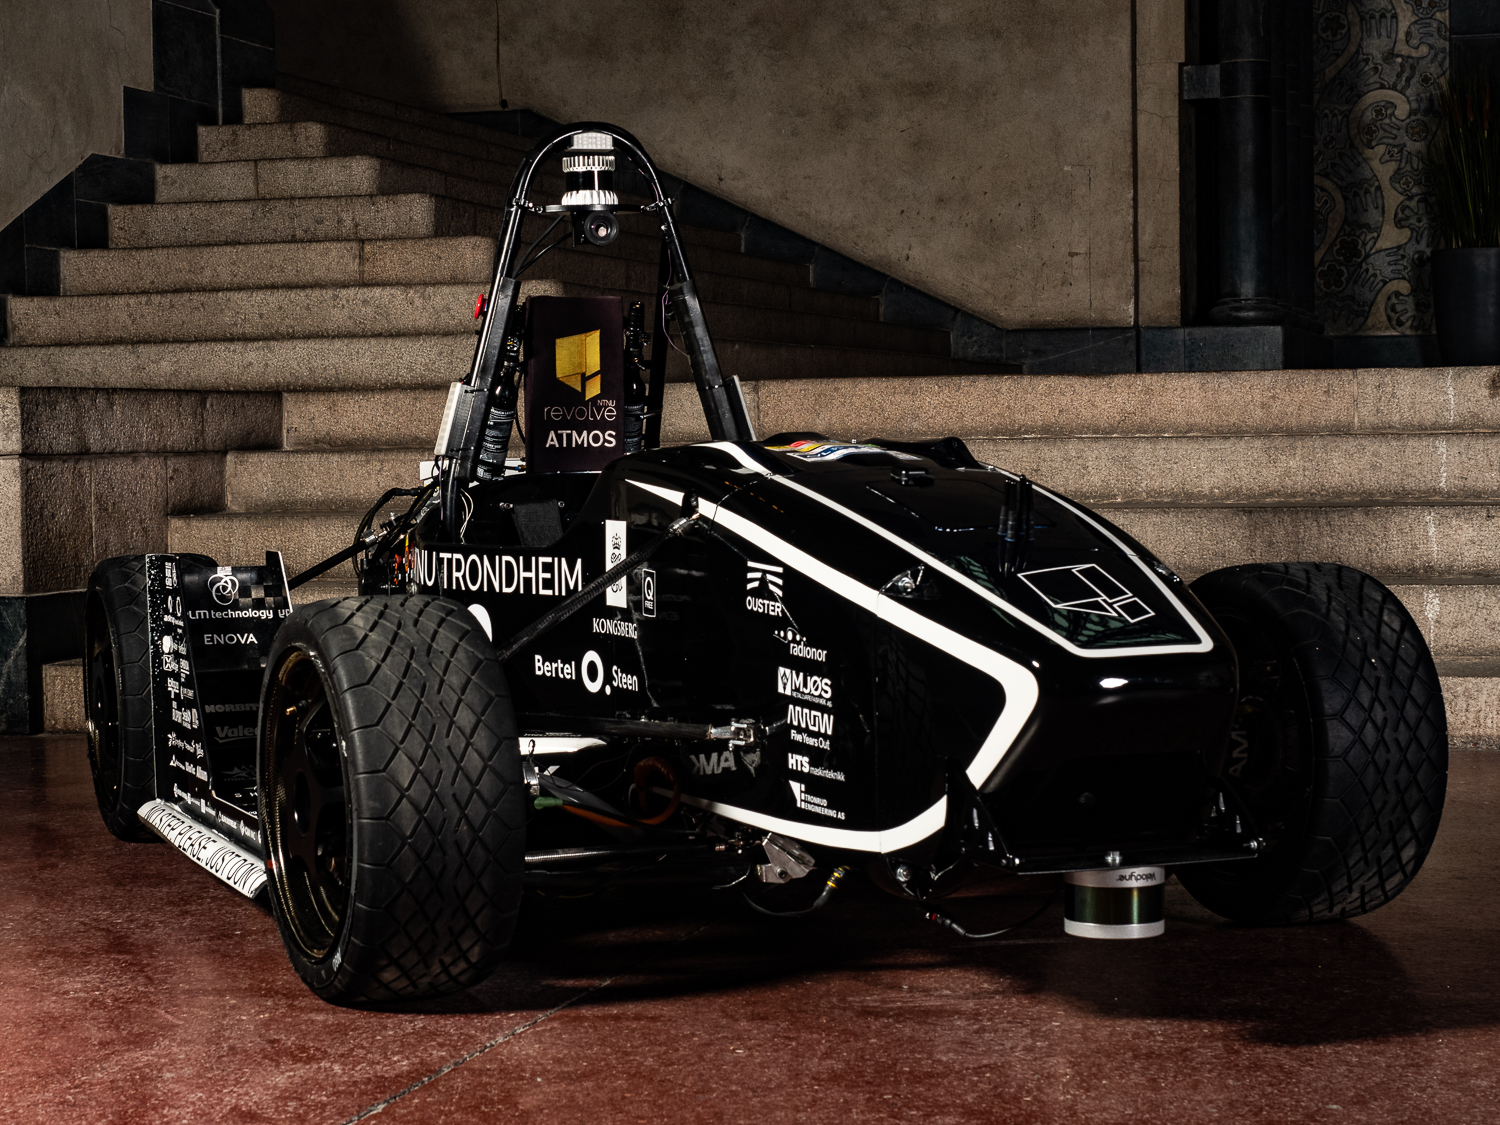
\includegraphics[width=\linewidth]{0_Images/2_Introduction/Atmos.jpg}
    \caption[Atmos.]{Atmos, Revolve NTNU's driverless car 2019.}
    \label{Fig:Atmos}
\end{figure}

\subsection{Nomenclature}

To establish a common language some of the nomenclature used at Revolve NTNU is first explained. 

A lot of the following discussion will deal with two main frames of references. One is the "base link" frame, sometimes referred to as the "body" frame. It is situated in the \gls{CG} of the car. The x-axis going in the longitudinal, the forward, direction of the car, its z-axis upwards away from the ground and its y-axis going in the left lateral direction, i.e. completing a right hand frame with the x- and the z-axis. This is illustrated in figure \ref{Fig:MapAndBodyFrames}. 

The other main frame is the "map" frame. It starts with the same position and orientation as the body frame when the car starts, but then remains fixed in the same pose relative to the earth fixed frame until the system is reset. This frame is also illustrated in figure \ref{Fig:MapAndBodyFrames}. 

Between these two frames lives another one; the odometry frame. The relationship between the map, odometry and body frames are illustrated in figure \ref{Fig:MapOdomAndBodyFrames}. 

\iffalse
\begin{figure}
    \centering
    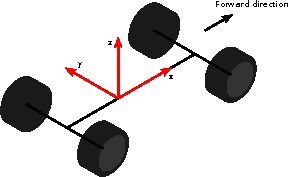
\includegraphics[width=0.5\linewidth]{0_Images/2_Introduction/BaseLinkScaled.pdf}
    \captionof{figure}{The "base link" or "body" frame.}
    \label{Fig:BodyFrame}
\end{figure}
\fi

\begin{figure}
    \centering
    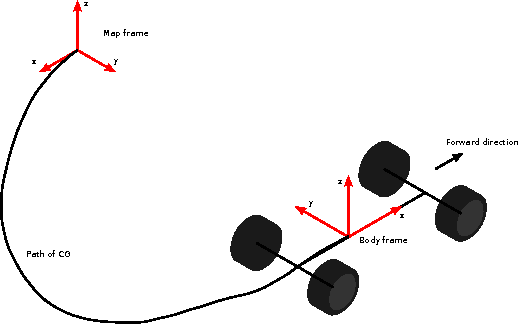
\includegraphics[width=0.5\linewidth]{0_Images/2_Introduction/MapAndBodyFrames.pdf}
    \captionof{figure}{The map and body frames.}
    \label{Fig:MapAndBodyFrames}
\end{figure}

\begin{figure}
    \centering
    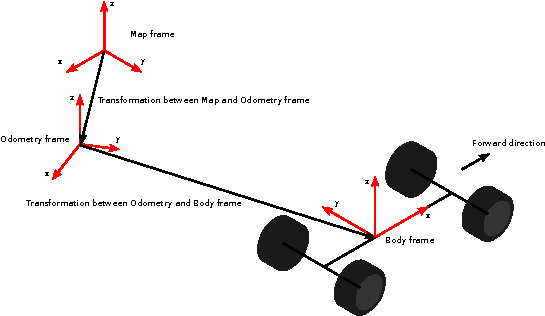
\includegraphics[width=0.5\linewidth]{0_Images/2_Introduction/MapOdomAndBodyFrames.pdf}
    \captionof{figure}{The relationship between the map, odometry and body frames.}
    \label{Fig:MapOdomAndBodyFrames}
\end{figure}

In the centre of each wheel is defined a reference frame, called the wheel frame. When the wheel is pointed straight ahead it has the same orientation as the body frame. This is illustrated in figure \ref{Fig:WheelFrame}. This frame will be important for talking about summing the forces from each wheel into one force and one torque on the CG. 

Furthermore it is beneficial to name a few of the components of the race car. The main hoop is the bent rod around the driver's head that saves him or her from being crushed by the car if it rolls over. The snout is the rounded tip of the front of the car. The track length of the car refers to the distance between the front and rear wheels along the x-axis, while the wheelbase is the distance between the right and left wheels along the y-axis. These terms are illustrated in figure \ref{Fig:NameOfCarParts}.

\begin{figure}
    \centering
    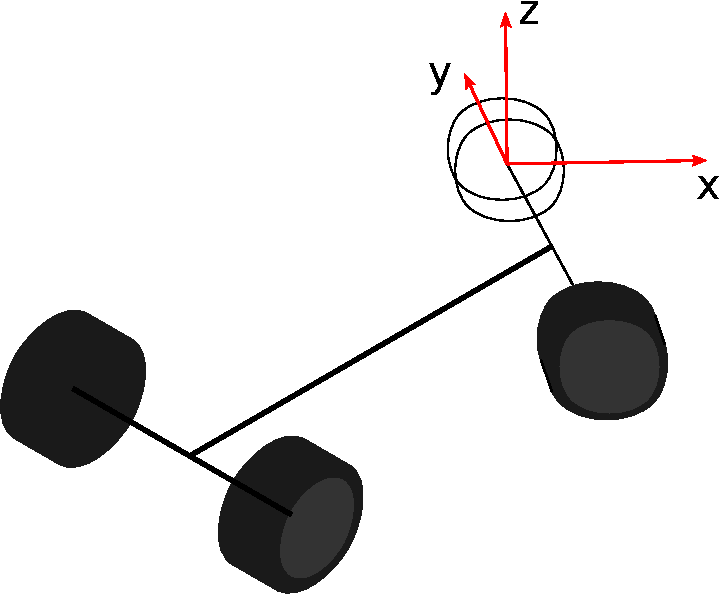
\includegraphics[width=0.5\linewidth]{0_Images/2_Introduction/WheelFrame.pdf}
    \captionof{figure}{Front left wheel frame. There are similar ones in the other three wheels.}
    \label{Fig:WheelFrame}
\end{figure}


\begin{figure}
    \centering
    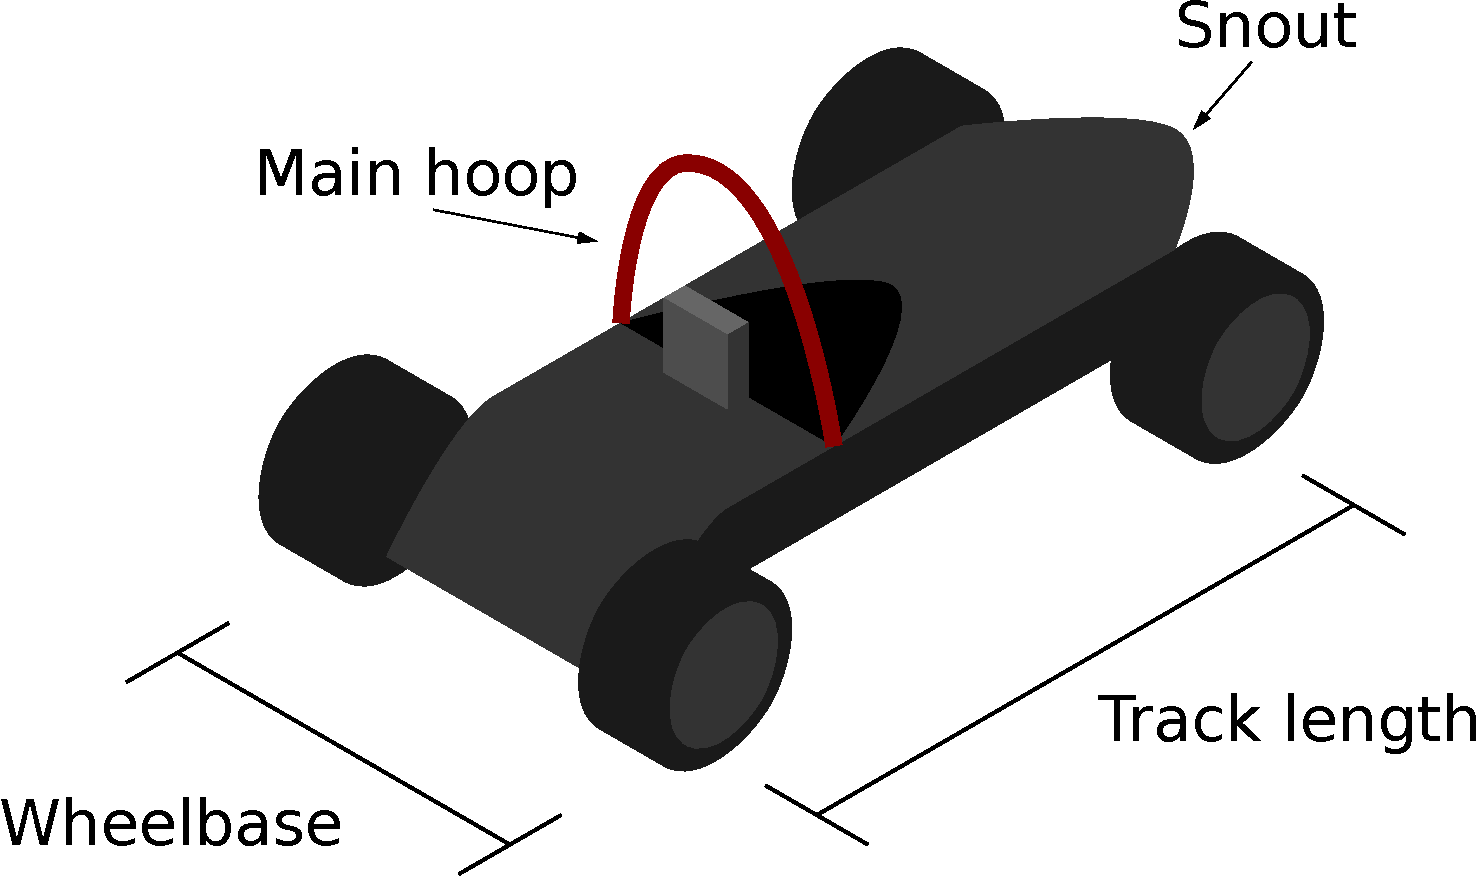
\includegraphics[width=0.5\linewidth]{0_Images/2_Introduction/NameOfCarParts.pdf}
    \captionof{figure}{Simple model of the car with names of some parts, along with illustrations of track length and wheelbase.}
    \label{Fig:NameOfCarParts}
\end{figure}
